\documentclass[12pt]{article}
\usepackage{geometry}                % See geometry.pdf to learn the layout options. There are lots.
\geometry{letterpaper}                   % ... or a4paper or a5paper or ... 
%\geometry{landscape}                % Activate for for rotated page geometry
\usepackage[parfill]{parskip}    % Activate to begin paragraphs with an empty line rather than an indent
\usepackage{daves,fancyhdr,natbib,graphicx,dcolumn,amsmath,lastpage,url}
\usepackage{amsmath,amssymb,epstopdf,longtable}
\usepackage{paralist}  % need to properly formulate standard answer blocks
\usepackage[final]{pdfpages}
\DeclareGraphicsRule{.tif}{png}{.png}{`convert #1 `dirname #1`/`basename #1 .tif`.png}
\pagestyle{fancy}
\lhead{CE 3305 Fluid Mechanics; Exercise Set 6}
\rhead{Name:\_\_\_\_\_\_\_\_\_\_\_\_\_\_\_\_\_\_\_\_\_\_\_\_\_\_\_\_\_\_\_\_\_\_}
\lfoot{REVISION A}
\cfoot{}
\rfoot{Page \thepage\ of \pageref{LastPage}}
\renewcommand\headrulewidth{0pt}
%%%%%%%%%%%%%%%%%%%%%%%%%%%%%%%%%%%%
\begin{document}
%%%%%%%%%%%%%%%%%%%%%%%%%%%%%%%%%%%
\begingroup
\begin{center}
{\textbf{{ CE 3305 Engineering Fluid Mechanics} \\ Exercise Set 6 \\ Summer 2018 -- GERMANY} }
\end{center}
\endgroup
\begingroup
~\newline
\textbf{Purpose} :  Application of static pressure to find forces on submerged plates. \\
\textbf{Assessment Criteria} : Completion, plausible solutions, use \textbf{R} as a calculator. \\~\\
\textbf{Exercises}

\begin{enumerate}
\item (Problem 3.70 pg 103)
Figure \ref{fig:SubmergedPanel} is a schematic of a panel at the bottom of a tank filled with water.  
The panel is square.  The distance from the free surface to the top of the panel is $d=1$ m, and $h=2$ m.   
\begin{enumerate}[a)]
\item Calculate the depth of the centroid.
\item Calculate the resultant force on the panel.
\item Calculate the distance from the centroid to the center of pressure (CP).
\end{enumerate}
\begin{figure}[htbp] %  figure placement: here, top, bottom, or page
   \centering
   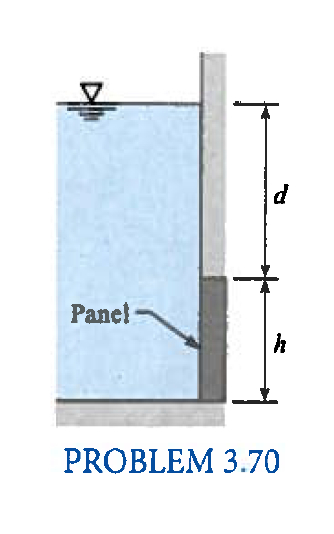
\includegraphics[width=2in]{SubmergedPanel.jpg} 
   \caption{Panel at bottom of a tank}
   \label{fig:SubmergedPanel}
\end{figure}
\clearpage
~

\item (Problem 3.74 pg 104)
Figure \ref{fig:HingeGate} is a schematic of a hinged gate with the hinge at the waterline.   
The gate is 4 ft high and 8 ft wide.  
The specific weight of water is 62.4 lbf/ft$^3$
Find the required force (in lbf) applied at the bottom of the gate to keep it shut.
\begin{figure}[htbp] %  figure placement: here, top, bottom, or page
   \centering
   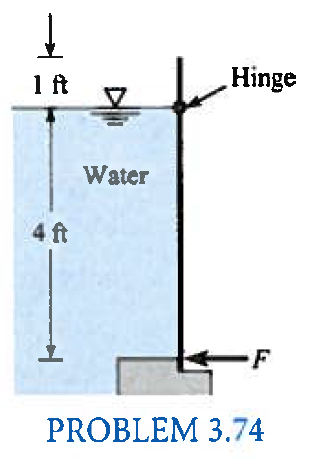
\includegraphics[width=2in]{HingeGate.jpg} 
   \caption{Hinged gate.}
   \label{fig:HingeGate}
\end{figure}

\end{enumerate}


\end{document}  